\chapter{Referencial Teórico}

O referencial teórico que sustentará este trabalho será explorado neste capítulo.
Para isso, foram feitas consultas de literatura utilizando \textit{strings} de busca na base científica Scopus, com foco nos principais conceitos que sustentam o tema deste trabalho.
A seguir estão listadas as palavras-chave e os rastros das consultas realizadas com elas:

\section{Palavras-chave}

Português:

\begin{itemize}
    \item Otimização de Aprendizado
    \item Gestão do Tempo
    \item Pomodoro
    \item Gamificação
    \item Cartões de Aprendizado
    \item Psicologia
    \item Motivação
    \item Estresse
    \item Ansiedade
    \item Metodologias de Aprendizado
\end{itemize}

Inglês:

\begin{itemize}
    \item \textit{Learning Optimization}
    \item \textit{Time Management}
    \item \textit{Pomodoro Technique}
    \item \textit{Gamification}
    \item \textit{Flashcards}
    \item \textit{Cards}
    \item \textit{Psychology}
    \item \textit{Motivation}
    \item \textit{Stress}
    \item \textit{Anxiety}
    \item \textit{Learning Methodologies}
\end{itemize}

\section{Rastros das Consultas}

Usando a \textit{string} de busca ("Learning Optimization" AND ("Gamification" OR "Spaced Repetition" OR "Pomodoro Technique")) foram retornados quatro artigos.
Lendo os títulos destes, foi escolhido o artigo de título:

\begin{itemize}
    \item \textit{Research AI: integrating AI and gamification in higher education for e-learning optimization and soft skills assessment through a cross-study synthesis}
\end{itemize}

Usando a \textit{string} de busca ("Time Management" AND "Academic Performance" AND "Study Strategy") foram retornados dezenove artigos.
Lendo os títulos destes, foram escolhidos os artigos de títulos:

\begin{itemize}
    \item \textit{Social Skills and Stress among Psychology, Nursing and Medical Students}
    \item \textit{Learning and study strategies correlate with medical students' performance in anatomical sciences}
    \item \textit{The relationship between study strategies and academic performance}
    \item \textit{Learning strategies, study habits and social networking activity of undergraduate medical students}
    \item \textit{Cognition, study habits, test anxiety, and academic performance}
\end{itemize}

Usando a \textit{string} de busca ("Psychology" AND ("Stress" OR "Anxiety") AND "Student" AND "Academic Achievement") foram retornados novecentos e três artigos.
Lendo os títulos dos vinte primeiros, foi escolhido o artigo de título:

\begin{itemize}
    \item \textit{Exploring the mediating role of anxiety between resilience and academic achievement in students' English learning}
\end{itemize}

Usando a \textit{string} de busca ("Time Management") foram retornados quinze mil quinhentos e quarenta artigos.
Lendo os títulos dos sessenta primeiros, foi escolhido o artigo de título:

\begin{itemize}
    \item \textit{Unlocking academic success: the impact of time management on college students' study engagement}
\end{itemize}

Usando a \textit{string} de busca ("Time Management" OR "Time Planning" OR "Time Management Skills") foram retornados dezenove mil duzentos e vinte artigos.
Lendo os títulos dos sessenta primeiros, foi escolhido o artigo de título:

\begin{itemize}
    \item \textit{Improving medical students' learning strategies, management of workload and wellbeing: a mixed methods case study in undergraduate medical education}
\end{itemize}

Usando a \textit{string} de busca ("learning methodology" OR "teaching method" OR "pedagogical approach") foram retornados sessenta e sete mil cento e quatorze artigos.
Lendo os títulos dos cinquenta primeiros, foram escolhidos os artigos de títulos:

\begin{itemize}
    \item \textit{Didactic methodologies used in police training schools to teach human rights}
    \item \textit{A comprehensive framework for higher education 4.0}
    \item \textit{Intelligent Technology-Driven Hybrid English Classroom Model for Enhanced Personalization and Learning Efficiency}
\end{itemize}

Usando a \textit{string} de busca ("Gamification" OR "Gamified Learning" OR "Game-Based Learning") foram retornados vinte e nove mil oitocentos e vinte artigos.
Lendo os títulos dos primeiros artigos, foram escolhidos os seguintes títulos:

\begin{itemize}
    \item \textit{Effects of game-based learning integrated with different thinking-guided methods on computational thinking of elementary school students}
    \item \textit{Gamified feedback in adaptive retrieval practice: Points and progress-bars enhance motivation but not learning}
\end{itemize}

Usando a \textit{string} de busca ("Spaced Repetition System") foram retornados treze artigos.
Lendo todos os títulos, foi escolhido o seguinte título:

\begin{itemize}
    \item \textit{Investigating the use of a mobile flashcard application rememba on the vocabulary development and motivation of EFL learners}
\end{itemize}

Usando a \textit{string} de busca ("self-regulated learning") foram retornados treze artigos.
Lendo todos os títulos, foi escolhido o seguinte título:

\begin{itemize}
    \item \textit{Promoting self-regulated learning during the covid-mandated remote learning period: Insights from interviews with primary school teachers}
\end{itemize}

Usando a \textit{string} de busca ("The Pomodoro Technique") foram retornados treze artigos.
Lendo todos os títulos, foi escolhido o seguinte título:

\begin{itemize}
    \item \textit{Assessing the efficacy of the Pomodoro technique in enhancing anatomy lesson retention during study sessions: a scoping review}
\end{itemize}

Usando a \textit{string} de busca ("software development methodologies") foram retornados mil setecentos e quarenta e um artigos.
Lendo os títulos dos vinte primeiros, foi escolhido o seguinte título:

\begin{itemize}
    \item \textit{From Traditional to Agile Methodologies in Software Project Management Education: A Case Study}
\end{itemize}

Usando a \textit{string} de busca ("Extreme Programming") foram retornados mil quinhentos e oitenta e dois artigos.
Lendo os títulos dos vinte primeiros, foi escolhido o seguinte título:

\begin{itemize}
    \item \textit{Implementation of Extreme Programming Method in Developing Website of Agribusiness Harvest Transportation Order Data Management}
\end{itemize}

Usando a \textit{string} de busca ("Scrum") foram retornados cinco mil setecentos e sessenta e sete artigos.
Lendo os títulos dos vinte primeiros, foi escolhido o seguinte título:

\begin{itemize}
    \item \textit{Applying Scrum to Knowledge Transfer Among Software Developers}
\end{itemize}

Usando a \textit{string} de busca ("Kanban") foram retornados dois mil seiscentos e quarenta e dois artigos.
Lendo os títulos dos vinte primeiros, foi escolhido o seguinte título:

\begin{itemize}
    \item \textit{Effect of the Kanban Method on Problem Based Learning applied to university students}
\end{itemize}

Usando a \textit{string} de busca ("Lean Inception") foram retornados doze artigos.
Lendo todos os títulos, foi escolhido o seguinte título:

\begin{itemize}
    \item \textit{Investigating Problem Definition and End-User Involvement in Agile Projects that Use Lean Inceptions}
\end{itemize}

Usando a \textit{string} de busca ("test-driven development") foram retornados mil cento e setenta e quatro artigos.
Lendo os títulos dos dez primeiros, foi escolhido o seguinte título:

\begin{itemize}
    \item \textit{On the use of Test-Driven Development for Embedded Systems}
\end{itemize}

Usando a \textit{string} de busca ("Software Requirements") foram retornados seis mil duzentos e noventa e quatro artigos.
Lendo os títulos dos cinquenta e um primeiros, foi escolhido o seguinte título:

\begin{itemize}
    \item \textit{Ensuring quality in software requirement engineering process: A comparative study}
\end{itemize}

Usando a \textit{string} de busca ("FURPS") foram retornados quarenta e dois artigos.
Lendo os títulos dos dez primeiros, foi escolhido o seguinte título:

\begin{itemize}
    \item \textit{Software Quality Attributes in Requirements Engineering}
\end{itemize}

Usando a \textit{string} de busca ("software architecture") foram retornados trinta e cinco mil cento e noventa e sete artigos.
Lendo os títulos dos cento e trinta primeiros, foi escolhido o seguinte título:

\begin{itemize}
    \item \textit{Editorial of the special issue on Quality in Software Architecture}
\end{itemize}

Usando a \textit{string} de busca ("UML") foram retornados vinte e três mil quatrocentos e sessenta e quatro artigos.
Lendo os títulos dos oitenta primeiros, foi escolhido o seguinte título:

\begin{itemize}
    \item \textit{A Research on the Impact of a Class Diagram Layout and Complexity on System Model Understandability}
\end{itemize}

Usando a \textit{string} de busca ("Entity-Relationship Model") com o filtro de acesso livre foram retornados cento e quarenta e sete artigos.
Lendo os títulos dos dez primeiros, foi escolhido o seguinte título:

\begin{itemize}
    \item \textit{Difficulties in understanding the transition between database design stages: An experiment from a semantic distance perspective}
\end{itemize}

Usando a \textit{string} de busca ("Logic Data Model") com o filtro de acesso livre foram retornados dois artigos.
Lendo todos os títulos, foi escolhido o seguinte:

\begin{itemize}
    \item \textit{Applying model-driven approach to building rapid distributed data services}
\end{itemize}

Além disso, foram coletados, em buscas na internet, dois livros de acesso livre para dar base às referências teóricas deste trabalho.
Seus títulos podem ser observados abaixo:

\begin{itemize}
    \item \textit{The Future of Software Quality Assurance}
    \item \textit{Handbook of Software Engineering Methods}
\end{itemize}

\section{Gestão do Tempo}

A gestão do tempo é um conceito fundamental no ambiente de preparação para provas, sendo definida como a disposição e a capacidade do indivíduo de planejar, agendar e executar atividades de estudo de forma eficáz.
Essa competência se define na habilidade do estudante de estabelecer metas, priorizar tarefas e otimizar o uso do tempo disponível.
Pesquisas demonstram que a disposição para o gerenciamento do tempo está diretamente associada ao engajamento nos estudos, sendo um fator importante para o sucesso acadêmico na jornada universitária \cite{fu_2025}.

Diante disso, em estudos realizados com estudantes, o componente de gestão do tempo se mostrou como um forte fator no desempenho acadêmico \cite{zhou_2016}. Portanto, a eficácia na gestão do tempo está diretamente ligada ao desempenho.
Isso sugere que o planejamento do tempo de estudo e o estabelecimento de rotinas são tão importantes para os resultados quanto as habilidades de autoavaliação e motivação.

Uma gestão de tempo eficiente contribui para o aumento do autocontrole do estudante, o que está ligado a um maior engajamento nos estudos \cite{fu_2025}.
Além disso, a definição de rotinas estruturadas previnem o uso de dispositivos móveis durante sessões de estudo, reforçando a ideia de que o planejamento ajuda a mitigar distrações e a manter-se focado.

A transição para o ambiente universitário, que torna necessário o estudo independente, coloca a gestão da carga de trabalho e o uso estratégico do tempo no centro das estratégias de aprendizagem.
Em cursos exigentes, a mudança dos métodos passivos de estudo para estratégias mais ativas exige que os estudantes aprimorem suas habilidades de autogestão \cite{harvey_2025}.
Assim, a gestão do tempo é uma estratégia de aprendizado que se torna necessária para que os alunos consigam adaptar-se à demanda da carga horária.

Finalmente, a gestão adequada do tempo se revela essencial para a manutenção do bem estar e para a prevenção de sobrecarga mental de estudantes.
A gestão da carga de trabalho, um componente do gerenciamento do tempo, é crucial para o bem estar dos estudantes, especialmente em ambientes de alta pressão \cite{harvey_2025}.
Quando os alunos dominam técnicas de organização do tempo, torna-se possível distribuir suas tarefas de forma mais equilibrada, reduzindo a sensação de ansiedade e estresse.

\section{Metodologias de Aprendizado}

A evolução dos ambientes de ensino superior implica diretamente na forma de se ensinar, migrando de abordagens centradas no professor para modelos pedagógicos focados no estudante.
Essa mudança é um dos pilares da chamada Educação Superior 4.0, que exige o desenvolvimento de competências, como a capacidade de resolução de problemas e o pensamento crítico \cite{amghar_2025}.
Tais metodologias buscam promover o engajamento ativo e a autonomia da jornada educacional, preparando os indivíduos para um mercado de trabalho dinâmico.

As metodologias ativas surgem como ferramentas para aprimorar a eficiência do aprendizado.
Um exemplo disso é o modelo de sala de aula híbrida impulsionado pela tecnologia, que visa otimizar o processo de ensino e fornecer suporte de aprendizagem \cite{wang_2026}.
Essas abordagens permitem que o conteúdo seja adaptado às necessidades e ao ritmo de cada aluno, superando as limitações dos métodos tradicionais de ensino presencial.

A escolha e a aplicação das metodologias didáticas devem ser adequadas ao conteúdo e aos objetivos, sendo importante a adoção de estratégias que estimulem a participação e a reflexão.
Em contextos específicos, como o treinamento policial em direitos humanos, a comunidade acadêmica sugere que as metodologias mais utilizadas incluem o estudo de casos, as conferências com especialistas e os grupos focais, que visam a sensibilização e a reflexão sobre valores éticos e princípios legais \cite{salazar_2026}.
A eficácia da metodologia está ligada à sua capacidade de mudar a técnica passiva do estudante para uma participação crítica no processo aprendizado.

\section{Gamificação}

A gamificação e a Aprendizagem Baseada em Jogos (\textit{Game-Based Learning} - GBL) representam uma área de estudo crescente, sendo reconhecidas como ferramentas capazes de potencializar o envolvimento e o interesse.
A GBL demonstrou ser uma metodologia eficáz para o desenvolvimento do pensamento computacional em estudantes do ensino fundamental \cite{hsu_2026}.
Esse tipo de abordagem transforma o processo de aprendizagem em uma experiência motivadora, integrando elementos de resolução de problemas por meio de cenários de jogo.

No entanto, o impacto da gamificação se manifesta majoritariamente na motivação, e normalmente não traz ganhos na aprendizagem em si.
Elementos gamificados, como sistemas de pontuação e barras de progresso, são altamente eficazes para aumentar a motivação e a persistência dos estudantes em estratégias de estudo que exigem esforço, como a prática de recuperação adaptativa \cite{vandenbroek_2026}.
Contudo, essa motivação não garante um aumento nos resultados destes estudos, apenas age como um positivo adicional à aprendizagem.

Para maximizar os benefícios da gamificação, é necessário que ela seja integrada a métodos de aprendizado eficázes.
A combinação do aprendizado baseado em jogos com métodos de orientação, como o 5W1H (o quê, quem, quando, onde, por que e como) ou o mapeamento de conceitos baseado em associação (CABCM), demonstrou ser eficáz na promoção do pensamento computacional e da autoeficácia de estudantes \cite{hsu_2026}.
Portanto, enquanto a gamificação fornece a estrutura motivacional, a inclusão de metodologias de aprendizado e de resolução de problemas é essencial para transformar esse engajamento em um resultado real.

\clearpage
\raggedbottom
\section{Aplicativos Similares}

Foi feita uma coleta de dados acerca de \textit{softwares} similares com objetivos análogos de auxiliar no fluxo de estudos de estudantes.

Um deles é o Aprovado, mostrado na Figura~\ref{fig:aprovado}, cujo seu propósito é atuar como uma ferramenta de produtividade e controle de tempo voltada para o estudante.
Seu principal recurso é o gerenciamento das horas de estudo, permitindo que o usuário registre o tempo dedicado a cada matéria, gerando gráficos e relatórios sobre a evolução e o desempenho nessas matérias.
Ao focar em métricas e estatísticas, o Aprovado se alinha com o pilar de gestão do tempo deste trabalho, fornecendo uma ideia de onde o tempo está sendo aplicado, o que é fundamental para a otimização da rotina de um estudante \cite{aprovado_2026}. Porém, o aplicativo não se concentra no campo da saúde mental do estudante e, logo, não trás uma visão da qualidade do estudo.

Dessa maneira, o Aprovado apresenta limitações ao ser comparado com o escopo do aplicativo proposto neste trabalho.
Enquanto o projeto visa uma solução completa que integra gestão do tempo, prática de recuperação ativa, gamificação e coleta de dados de bem estar, o Aprovado é majoritariamente uma ferramenta de controle de horas.

\begin{figure}[H]
    \centering
    \caption{Tela inicial do Aprovado}
    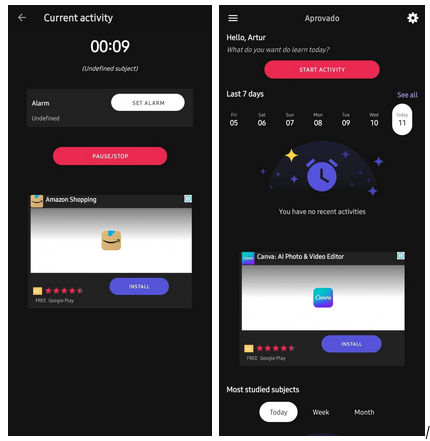
\includegraphics[width=0.75\linewidth]{Imagens/Aprovado.png}
    \par
    Fonte: \cite{aprovado_2026}.
    \par
    \label{fig:aprovado}
\end{figure}

De outra maneira, o StudyTok, mostrado na Figura~\ref{fig:studytok}, é uma plataforma mais dinâmica, utilizando a Inteligência Artificial (IA) para transformar materiais de estudo em componentes dentro da aplicação.
Seu principal valor é a funcionalidade de geração de material de estudo, em que o usuário envia imagens, PDFs, PowerPoints e vídeos para o aplicativo e, em seguida a IA gera questionários e \textit{flashcards}.
Essa funcionalidade está diretamente ligada ao valor da prática de recuperação ativa, permitindo que a IA crie os recursos necessários para a repetição espaçada ao invés do próprio aluno, otimizando o tempo que seria gasto na criação manual \cite{studytok_2026}.

Além disso, o aplicativo possui a gamificação através de placares de líderes e um sistema de recompensa por pontos a fim de manter a motivação do usuário. Portanto, em comparação com este trabalho, o StudyTok não possui os valores de gestão do tempo e controle da saúde mental que este trabalho pretende implementar \cite{studytok_2026}.

\begin{figure}[H]
    \centering
    \caption{Tela inicial do StudyTok}
    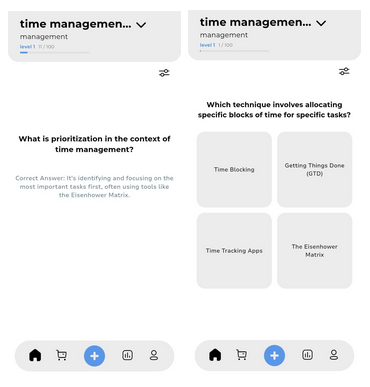
\includegraphics[width=0.75\linewidth]{Imagens/StudyTok.png}
    \par
    Fonte: \cite{studytok_2026}.
    \par
    \label{fig:studytok}
\end{figure}

Portanto, o aplicativo proposto para este trabalho se diferencia dos concorrentes ao buscar uma integração completa de todos os valores mencionados anteriormente.
Enquanto o Aprovado se restringe ao registro e à estatística da gestão do tempo e o StudyTok se destaca na geração de \textit{flashcards} por IA e gamificação, o aplicativo proposto visa combinar esses valores com o controle de bem estar a fim de trazer um produto centralizado e desfragmentado.
O diferencial está em combinar a eficácia da repetição espaçada com uma ferramenta de cronômetro Pomodoro, elementos de gamificação e \textit{check-ins} de humor, oferecendo assim uma solução mais coesa e adaptada às demandas do estudante.

\flushbottom
\clearpage
\section{Heurísticas de Nielsen}

A boa usabilidade de um sistema é construída a partir de um conjunto de regras reconhecidas no campo da engenharia de \textit{software} como as heurísticas de Nielsen.
São dez princípios que servem como um guia para a implementação de interfaces digitais centradas nas necessidades do usuário.
As heurísticas visam garantir que o sistema não apenas funcione, mas que seja acessível e fácil de usar.

Segundo essas diretrizes, o sistema deve: (i) sempre manter o usuário informado sobre o que está acontecendo, com \textit{feedbacks}; (ii) usar linguagens conhecidas pelo usuário enquanto segue convenções já estabelecidas; (iii) oferecer oportunidades de cancelamento de operações indesejadas; (iv) os elementos do aplicativo devem se comportar de forma semelhante; (v) evitar erros antes que eles surgam; (vi) tornar objetos, ações e opções visíveis; (vii) incluir atalhos para usuários experientes; (viii) excluir componentes com informações irrelevantes; (ix) informar especificamente qual erro ocorreu, em sua mensagem; e (x) implementar uma documentação de auxílio.

Dessa forma, este trabalho se compromete a aplicar rigorosamente essas heurísticas para garantir a usabilidade e a acessibilidade para todos os públicos.
Além disso, o projeto respeita a Lei Geral de Proteção de Dados (LGPD) \cite{brasil2018lgpd}, garantindo segurança, privacidade e transparência no tratamento das informações dos usuários.

\section{Algoritmo de Repetição Espaçada (ARE)}

A metodologia do algoritmo de repetição espaçada (ARE) foca na ideia da memorização de longo prazo, buscando otimizar o tempo de estudo ao confrontar a curva do esquecimento.
Diante disso, o ARE sempre calcula um intervalo de revisão adequado para o usuário conforme a dificuldade, apresentando o conteúdo no momento em que estaria sendo esquecido, o que é mais eficaz comparado com a repetição excessiva.
A implementação dessa metodologia ganhou populariedade em aplicações móveis, pois a portabilidade dos \textit{smartphones} eliminam os problemas de tempo e local, permitindo que estudantes estudem quando e onde quiserem.
Nesse contexto, estudos como o de \citeonline{kose_2018} investigaram os efeitos de uma aplicação de \textit{flashcards} móveis com sistema de repetição espaçada sobre o desenvolvimento do vocabulário e a motivação dos estudantes, demonstrando que essa implementação resulta em aumentos mais altos de vocabulário e maior motivação.

Os algoritmos de repetição espaçada se classificam como uniforme ou dinâmico, este sendo mais eficiente já que calcula o tamanho ideal do intervalo da repetição conforme o \textit{feedback}.
O objetivo desses algoritmos, especialmente o espaçamento dinâmico, é capacitar os estudantes a dedicarem mais tempo aos itens que exigem mais sessões de revisão e menos tempo àqueles que já estão consolidados.

\section{Pomodoro \textit{Timer}}

O  cronômetro Pomodoro é uma metodologia de gestão do tempo que estrutura o trabalho ou estudo em intervalos de foco, intercalados com pausas curtas e obrigatórias, com o objetivo de aumentar a produtividade e evitar a fadiga.
Criada por Francesco Cirillo, a técnica divide o tempo em intervalos de 25 minutos de foco, seguidos por 5 minutos de descanso.
A cada quatro ciclos completos, há uma pausa de 30 minutos.
Essa abordagem se alinha com o valor de gestão do tempo deste trabalho, proporcionando ao estudante uma metodologia eficaz para ajudar no planejamento e execução das tarefas.

O cronômetro Pomodoro gera o incentivo de descanso na hora ideal a fim de ajudar na manutenção da atenção.
Ao garantir pausas frequentes, a técnica permite que a pessoa se recupere, evitando a sobrecarga e o declínio na retenção de informações.
Dessa forma, a relevância dessa metodologia é crescente, com pesquisas que buscam avaliar sua aplicabilidade em campos de estudos.
Um exemplo disso é a revisão de escopo realizada por \citeonline{ogut_2025}, que teve como objetivo avaliar a relevância da técnica Pomodoro na retenção de lições de anatomia demonstrando a busca por evidências da eficácia da técnica em ambientes acadêmicos.
O estudo aponta que mesmo intervalos estruturados como 24 minutos de trabalho seguidos por 6 minutos de descanso ou 12 minutos de trabalho seguidos por 3 minutos de descanso levaram a resultados positivos em provas.
Dessa forma, será implementado a funcionalidade de um cronômetro Pomodoro com ciclos configuráveis, permitindo que o usuário ajuste os tempos de foco e pausa de acordo com sua preferência.

\section{Aprendizagem Autorregulada (\textit{Check-ins} de Humor)}

A aprendizagem autorregulada (\textit{Self-Regulated Learning} - SRL) descreve o processo pelo qual os estudantes monitoram e controlam seu aprendizado.
A capacidade de autorregulação permite que o estudante ajuste seu comportamento e planejamento de estudo em resposta às demandas e ao seu estado mental.
Essa importância se tornou ainda mais evidente em contextos de estudo autodidata, como o ensino remoto causado pela COVID-19, onde o suporte do professor foi limitado, exigindo maior independência do aluno.

O estado psicológico do estudante impacta diretamente a absorção de informação e o engajamento com a tarefa.
A metodologia SRL diz que, se o estudante está ciente de que seu humor está baixo ou seu estresse alto, ele pode usar estratégias de autorregulação para mitigar esse efeito negativo, como ajustar a dificuldade da tarefa, alterar o foco de estudo ou tirar uma pausa.
O estudo de \citeonline{ebbes_2026}, ao entrevistar professores sobre o ensino remoto, destacou que um dos principais desafios enfrentados pelos educadores era justamente o suporte ao bem estar emocional dos alunos.

Dessa forma, a integração de \textit{check-ins} de bem estar e a análise dos gráficos gerados transformam o aplicativo em um agente de suporte à SRL.
Ao coletar dados sobre o estado emocional, o sistema pode oferecer uma oportunidade de análise desses índices, permitindo o surgimento de ideias de intervenção que promovem a saúde mental e otimizam a produtividade.
Essa funcionalidade metodológica atende diretamente à necessidade, identificada em pesquisas como a de \citeonline{ebbes_2026}, de monitorar o engajamento e o bem estar emocional do aluno em um ambiente de estudo individual, atuando como um professor que oferece esse suporte.
